\section{Statistics}

\begin{definition}[Bernoulli distribution]\label{bernoulli}
    A distribution of parameters, where $\forall x, 0 \leq x \leq 1$,
    Typically dual, e.g.\ in coin toss there is heads and tails.
    If $\Pr_{heads} = k$, then $\Pr_{tails} = 1 - \Pr_{heads}$
\end{definition}

\begin{definition}[Bigvee]
    $\bigvee\limits_{a \in I} P_{a}$ says that at least one $P_{a}$ is true.
    It can also be used for the maximum value in a set.
\end{definition}

\begin{definition}[Central moment]
    The distribution of variable $[$values$]$ around the mean. 
    This way, you can now if the distribution is spread out or not.

\end{definition}

\begin{definition}[Cauchy distribution] 
    A family of distributions with no expected value.
    They usually look like:

    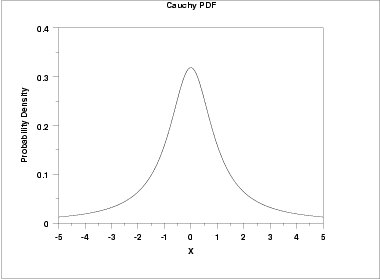
\includegraphics[scale=.5]{cau.png}

\end{definition}

\begin{definition}[Chernoff bound]\label{chernoff}
    In a nutshell, it determines a bound on how many times we must perform
    a trial to know that our random variables represent a majority.
    E.g.\ if we trying to determine that a coin is biased (heads/tails),
    a chernoff bound will say how many times we must flip the coin to know
    that we have unraveled a bias. In this case, for example, simply flipping it
    twice will not suffice.
\end{definition}

\begin{definition}[Conditional expectations]
    $$
        E(X | Y=y) = \sum\limits_{x \in X} x \
        P(X=x | Y=y) = \sum_{x \in X} x 
        \frac{P(X=x,Y=y)}{P(Y = y)}
    $$
\end{definition}

\begin{definition}[Conditional probability]
    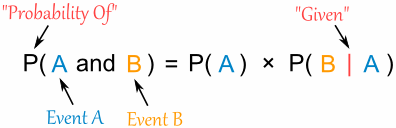
\includegraphics[scale=0.3]{prob_form.png}
\end{definition}

\begin{definition}[Covariance]
    A measure of how much two random variables change together.

\end{definition}

\begin{definition}[Expected value]\label{expectedvalue}
    $E[X] = \sum\limits_{s \in S}^{\dots} X(s) \cdot \Pr(\{s\}) $ \newline
    $E[X] = \sum\limits_{s \in S}^{\dots} X(s) \cdot \Pr(X = x) $
\end{definition}

\begin{definition}[hyperplane]
    A plane (surface) that has one less dimension than it's ambient space,
    i.e.\ the space around it. E.g.\ a hyperplane for 3-d dims is only defined
    2D.

    A hyperplane will therefore act as a separator. Imagine a holding a 
    square in the middle of a ball.
\end{definition}

\begin{definition}[Gold standard]
In medicine and statistics, gold standard test refers to a diagnostic test or
benchmark that is the best available under reasonable conditions. It does
not have to be necessarily the best possible test for the condition in absolute
terms. For example, in medicine, dealing with conditions that require an
autopsy to have a perfect diagnosis, the gold standard test is less accurate
than the autopsy.

\end{definition}

\begin{definition}[Ground truth]
    to the accuracy of the training set's classification for supervised
    learning techniques. This is used in statistical models to prove or
    disprove research hypotheses. The term "ground truthing" refers to the
    process of gathering the proper objective data for this test.

\end{definition}

\begin{definition}[Normal (Gaussian) distribution]
    A distribution that is centered around a value.
    E.g.\ when you collect people's height, there will be many around the
    average, and fewer and fewer to the sides.

\end{definition}

\begin{definition}[Indicator variable]
    Indicator variable: 0 or 1 for whether an element is selected or not.
\end{definition}


\begin{definition}[Linearity of expectation]\label{lin_expect}
    $ E[X] + E[Y] = E[X + Y] \newline
    [\sum\limits_{x \in S}^{\dots} X(s) \cdot \Pr(X = x) +
    \sum\limits_{y \in S}^{\dots} X(s) \cdot \Pr(Y = y) ] \newline
    = [\sum\limits_{s \in S}^{\dots} a \cdot \Pr(Y = a) + a \cdot \Pr(X = a) ]
    $
\end{definition}

\begin{theorem}[Likelyhood that both X and Y occur in S]
    $ \newline E[X] \cdot E[Y] = E[X \cdot Y]$
\end{theorem}
\begin{proof}
    From~\nameref{expectedvalue}: \newline
    $
    E[X \cdot Y] = \newline \sum\limits_{z \in S}^{\dots} z \cdot 
        \Pr(X = z \text{ and } Y = z) = \newline
    \sum\limits_{x \in S}^{\dots}\sum\limits_{y \in S}^{\dots} x \cdot y
    \cdot \Pr(X = x \text{ and } Y=y) = \newline
    [\sum\limits_{x \in S}^{\dots} x \cdot \Pr(X = x)] \cdot  
    [\sum\limits_{y \in S}^{\dots} y \cdot \Pr(Y = y)]  = \newline
    E[X] \cdot E[Y]
    $
\end{proof}


\begin{definition}[Markov Property]
    Memoryless stochastic process - what happened at point of time X
    does not matter for times $Y \geq X$.
\end{definition}

\begin{definition}[Poisson distribution]
    expresses the probability of a given number of events occurring in a fixed
    interval of time and/or space if these events occur with a known average
    rate and independently of the time since the last even.

\end{definition}

\begin{definition}[Probability Mass function]
    A function that gives a probability that a variable is exactly equal to
    some value.
\end{definition}

\begin{definition}[Supervised learning]
    the machine learning task of inferring a function from labeled training
    data. The training data consist of a set of training examples. In
    supervised learning, each example is a pair consisting of an input object
    (typically a vector) and a desired output value (also called the
    supervisory signal).

\end{definition}
